\documentclass{article}
\usepackage{amsmath}
\usepackage[top=2cm, left=2cm, right=1cm, bottom=2cm]{geometry}
\usepackage{fancyhdr}
\usepackage{graphicx}
\usepackage{longtable}

\usepackage{amsmath,amssymb}
\usepackage{iftex}
\ifPDFTeX
  \usepackage[T1]{fontenc}
  \usepackage[utf8]{inputenc}
  \usepackage{textcomp} % provide euro and other symbols
\else % if luatex or xetex
  \usepackage{unicode-math} % this also loads fontspec
  \defaultfontfeatures{Scale=MatchLowercase}
  \defaultfontfeatures[\rmfamily]{Ligatures=TeX,Scale=1}
\fi
\usepackage{lmodern}
\ifPDFTeX\else
  % xetex/luatex font selection
\fi
% Use upquote if available, for straight quotes in verbatim environments
\IfFileExists{upquote.sty}{\usepackage{upquote}}{}
\IfFileExists{microtype.sty}{% use microtype if available
  \usepackage[]{microtype}
  \UseMicrotypeSet[protrusion]{basicmath} % disable protrusion for tt fonts
}{}
\makeatletter
\@ifundefined{KOMAClassName}{% if non-KOMA class
  \IfFileExists{parskip.sty}{%
    \usepackage{parskip}
  }{% else
    \setlength{\parindent}{0pt}
    \setlength{\parskip}{6pt plus 2pt minus 1pt}}
}{% if KOMA class
  \KOMAoptions{parskip=half}}
\makeatother
\usepackage{xcolor}
\usepackage{longtable,booktabs,array}
\usepackage{calc} % for calculating minipage widths
% Correct order of tables after \paragraph or \subparagraph
\usepackage{etoolbox}
\makeatletter
\patchcmd\longtable{\par}{\if@noskipsec\mbox{}\fi\par}{}{}
\makeatother
% Allow footnotes in longtable head/foot
\IfFileExists{footnotehyper.sty}{\usepackage{footnotehyper}}{\usepackage{footnote}}
\makesavenoteenv{longtable}
\usepackage{graphicx}
\makeatletter
\def\maxwidth{\ifdim\Gin@nat@width>\linewidth\linewidth\else\Gin@nat@width\fi}
\def\maxheight{\ifdim\Gin@nat@height>\textheight\textheight\else\Gin@nat@height\fi}
\makeatother
% Scale images if necessary, so that they will not overflow the page
% margins by default, and it is still possible to overwrite the defaults
% using explicit options in \includegraphics[width, height, ...]{}
\setkeys{Gin}{width=\maxwidth,height=\maxheight,keepaspectratio}
% Set default figure placement to htbp
\makeatletter
\def\fps@figure{htbp}
\makeatother
\setlength{\emergencystretch}{3em} % prevent overfull lines
\providecommand{\tightlist}{%
}
\setcounter{secnumdepth}{-\maxdimen} % remove section numbering
\ifLuaTeX
  \usepackage{selnolig}  % disable illegal ligatures
\fi
\usepackage{bookmark}
\IfFileExists{xurl.sty}{\usepackage{xurl}}{} % add URL line breaks if available
\urlstyle{same}
\hypersetup{
  hidelinks,
  pdfcreator={LaTeX via pandoc}}


\begin{document}
\pagestyle{fancy}
\fancyhf{}
\lfoot{Test ID: 2048}
\rfoot{Page: \thepage}
\renewcommand{\footrulewidth}{0.4pt}

\noindent
\textbf{Instructions:} Questions 1-14 are multiple choice. For each problem, circle the letter of the best answer.
You \textbf{must show all work} for credit. Partial credit may be awarded as appropriate. Each question is
valued at 3 points.
\begin{enumerate}
	\itemsep2em
	\item
	\begin{minipage}[t]{\linewidth}
		If \(y=6 \ln (3 x)\) then what is \(y^{\prime}\) ?\\[0.1em]
		\begin{enumerate}
		\itemsep1em
			\item  $\dfrac{2}{x}$
			\item  $\dfrac{6}{x}$

			\item  $\dfrac{1}{3x}$
			\item  $\dfrac{18}{x}$
		\end{enumerate}
	\end{minipage}
	\item
	\begin{minipage}[t]{\linewidth}
		What is the value of

\[
\lim _{\Delta x \rightarrow 0} \frac{2(x+\Delta x)^{2}-2 x^{2}}{\Delta x}
\]\\[0.1em]
		\begin{enumerate}
		\itemsep1em
		\item  $4 x$

			\item  $2 x$
			\item  4
			\item  2
		\end{enumerate}
	\end{minipage}
	\item
	\begin{minipage}[t]{\linewidth}
		If \(w(t)=\sqrt{t^{2}-1}\) what is the value of \(w^{\prime}(4)\) ?\\[0.1em]
		\begin{enumerate}
		\itemsep1em
			\item  $\dfrac{2}{\sqrt{15}}$
			\item  $\dfrac{1}{\sqrt{15}}$
			\item  $\dfrac{1}{2 \sqrt{15}}$
			\item  $\dfrac{4}{\sqrt{15}}$
		\end{enumerate}
	\end{minipage}
	\item
	\begin{minipage}[t]{\linewidth}
		At which \(x\) value does the graph of \(y=3 x^{2}-10 x+15\) have a
horizontal tangent line?\\[0.1em]
		\begin{enumerate}
		\itemsep1em
			\item  $\dfrac{-3}{5}$
			\item  $\dfrac{3}{5}$
			\item  $\dfrac{-5}{3}$
			\item  $\dfrac{5}{3}$
		\end{enumerate}
	\end{minipage}
	\item
	\begin{minipage}[t]{\linewidth}
		If \(h(x)=f\left(x^{2}+1\right)\) then which of the following is true?\\[0.1em]
		\begin{enumerate}
		\itemsep1em
			\item  $h^{\prime}(x)=f^{\prime}(2 x)$
			\item  $h^{\prime}(x)=2 x f^{\prime}(2 x)$
			\item  $h^{\prime}(x)=2x f^{\prime}\left(x^{2}+1\right)$

			\item  $h^{\prime}(x)=f^{\prime}\left(x^{2}+1\right)$
		\end{enumerate}
	\end{minipage}
	\item
	\begin{minipage}[t]{\linewidth}
		If \(f(x)=\sin \left(2x +1\right)\) and \(g(x) = f^{\prime}(x)\), find
\(g^{\prime}(x)\)\\[0.1em]
		\begin{enumerate}
		\itemsep1em
			\item  $g^{\prime}(x) = 2 \sin (2x + 1)$
			\item  $g^{\prime}(x) = -4 \sin (2x + 1)$

			\item  $g^{\prime}(x) = 4 \sin(2x + 1) \cos(2x + 1)$
			\item  $g^{\prime}(x) = -4x \cos(2x + 1)$
		\end{enumerate}
	\end{minipage}
	\item
	\begin{minipage}[t]{\linewidth}
		The graph of a continuous differentiable function \(f\) is shown
below.\\
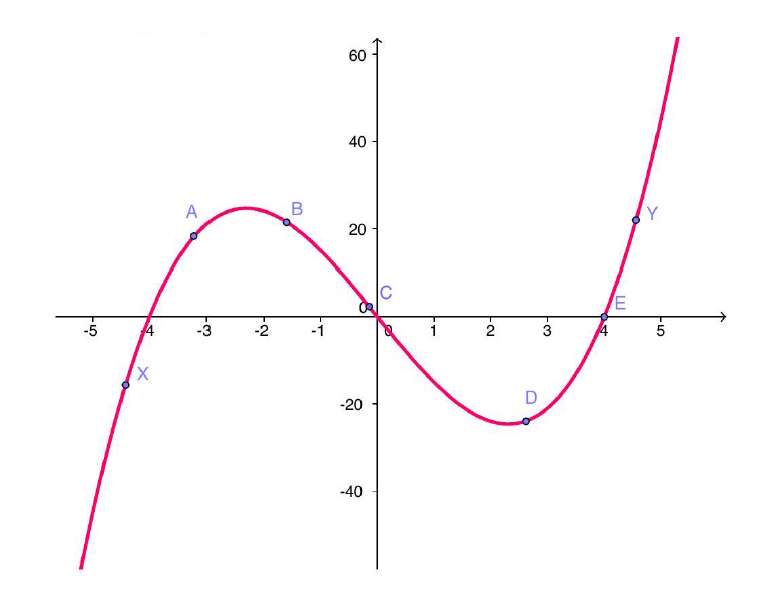
\includegraphics[width=0.6\textwidth,height=\textheight]{graph1.PNG}\\
Using the above graph, select the one true statement below.\\[0.1em]
		\begin{enumerate}
		\itemsep1em
		\item  $f'(C) < f'(D) < f'(Y)$
			\item  $f'(A) < f'(B) < f'(C)$
			\item  $f'(X) < f'(Y) < f'(C)$
			\item  $f'(X) < f'(B) < f'(E)$
		\end{enumerate}
	\end{minipage}
	\item
	\begin{minipage}[t]{\linewidth}
		Let \(f(x)=x^{3}-6 x^{2}+10\). At which point(s) on the graph of \(f\)
is the tangent line parallel to the line \(15 x-y=11\) ?\\[0.1em]
		\begin{enumerate}
		\itemsep4em
			\item  $(2,-6)$ and $(-2,22)$
			\item  $(5,-15)$ and $(-1,3)$
			\item  $(2,-6)$ and $(-2,-22)$
			\item  $(5,-15)$ and $(2,-6)$
		\end{enumerate}
	\end{minipage}
	\item
	\begin{minipage}[t]{\linewidth}
		If \(y(x) = \dfrac{\sin(2x)}{x^2}\) find \(y'(x)\)\\[0.1em]
		\begin{enumerate}
		\itemsep1em
		\item  $\dfrac{2 x \cos(2 x) - 2 \sin(2 x)}{x^3}$

			\item  $\dfrac{ 2 \cos(2x)}{x}$
			\item  $\dfrac{ x^2 \cos(2x) - \sin(2x)} { x^3}$
			\item  $\dfrac{ x^2 \sin(2x) + 2 \cos(2x)} {x^4}$
		\end{enumerate}
	\end{minipage}
	\item
	\begin{minipage}[t]{\linewidth}
		Calculate \(\dfrac{d}{dt} \left( \ln(e^{2t}) - 2t \right)\)\\[0.1em]
		\begin{enumerate}
		\itemsep1em
		\item  0
			\item  $\dfrac{1}{2t}-2$
			\item  $\dfrac{2}{e^{2t}}-2$
			\item  $\dfrac{1}{2e^{2t}}-2$
		\end{enumerate}
	\end{minipage}
	\item
	\begin{minipage}[t]{\linewidth}
		Let \(f(x)=\sqrt{x}\). What is the equation of the tangent line to \(f\)
at the point \((4,2)\)?\\[0.1em]
		\begin{enumerate}
		\itemsep1em
			\item  $y=-\frac{1}{2} x+3$
			\item  $y=\frac{1}{4} x+1$

			\item  $y=\frac{1}{2} x$
			\item  $y=2 x-6$
		\end{enumerate}
	\end{minipage}
	\item
	\begin{minipage}[t]{\linewidth}
		What is the derivative of \(s(t)=\cos \left(t^2 + 1\right)\) ?\\[0.1em]
		\begin{enumerate}
		\itemsep1em
			\item  $-(t^2+1)\sin(t^2+1)$
			\item  $\cos(2t)$
			\item  $-2t\sin(t^2+1)$

			\item  $-\sin(2t)$
		\end{enumerate}
	\end{minipage}
	\item
	\begin{minipage}[t]{\linewidth}
		If \(f\) and \(h\) are nonzero differentiable functions, then the
derivative of \(\dfrac{f}{h}\) is\\[0.1em]
		\begin{enumerate}
		\itemsep1em
		\item  $\dfrac{f^{\prime} h - f h^{\prime}}{h^2}$

			\item  $\dfrac{f^{\prime} h + f h^{\prime}}{h^2}$
			\item  $\dfrac{f h^{\prime} - f^{\prime} h}{h^{2}}$
			\item  $\dfrac{f^{\prime}}{h^{\prime}}$
		\end{enumerate}
	\end{minipage}
	\item
	\begin{minipage}[t]{\linewidth}
		The line tangent to the curve \(y=\sqrt{16-x}\) at the point \((0,4)\)
has slope\\[0.1em]
		\begin{enumerate}
		\itemsep1em
			\item  4
			\item  $\dfrac{1}{8}$
			\item  $-4$
			\item  $\dfrac{-1}{8}$
		\end{enumerate}
	\end{minipage}

\end{enumerate}

	\begin{minipage}[t]{\linewidth}
		\textbf{Free Response Section:} Selected values of \(f, g, f', g'\) are given in the table below. \\
		\renewcommand{\arraystretch}{2}

			\begin{center}
				\begin{tabular}{|c|c|c|c|c|c|}
				\hline
				$x$ & 0 & 1 & 2 & 3 & 4 \\
				\hline
				$f(x)$ & $\frac{1}{2}$ & $\frac{1}{3}$ & 1 & -1 & 3 \\[0.5em]
				\hline
				$g(x)$ & -2 & 1 & $-\frac{1}{2}$ & 2 & $-\frac{1}{3}$ \\
				\hline
				$f^{\prime}(x)$ & $\frac{3}{2}$ & $\frac{5}{3}$ & $\frac{1}{4}$ & 0 & $-\frac{4}{5}$ \\
				\hline
				$g^{\prime}(x)$ & -1 & $\frac{2}{3}$ & -4 & -3 & $-\frac{1}{3}$ \\
				\hline
				\end{tabular}
				\end{center}
			\vspace{2em}
			Using the values in the table, evaluate the following derivatives. \textbf{You
			must show the symbolic derivative as the first part of your answer for credit!}\\[0.1em]
					\begin{enumerate}
					\setcounter{enumi}{14}
					\itemsep1em
					  \item  $\dfrac{d}{dx} \left( f(x) + g(x) \right)$ at $x=4$ \vspace{0.9in}
						\item  $\dfrac{d}{dx} \left( f(x)g(x) \right)$ at $x = 1$ \vspace{0.9in}
						\item  $\dfrac{d}{dx} \left( \dfrac{f(x)}{g(x)} \right)$ at $x = 0$ \vspace{0.9in}
						\item  $\dfrac{d}{dx} \left( f(g(x)) \right)$ at $x = 3$ \vspace{0.9in}
						\item  $\dfrac{d}{dx} \left( g(x+f(x)) \right)$ at $x = 3$ \vspace{0.9in}
					\end{enumerate}
				\end{minipage}



\end{document}
